% 2006_jiangxi_science_q20_fig1: tetrahedron A-BCD, BD hidden dashed
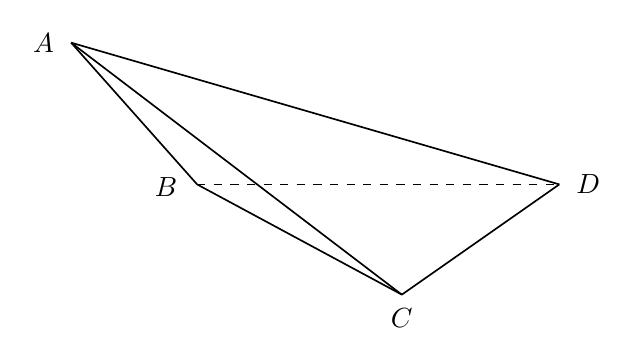
\begin{tikzpicture}[x=1cm,y=1cm,font=\normalsize,
  geometry edge/.style={solid,line width=.6pt},
  geometry label/.style={font=\normalsize,inner sep=2pt}]
\coordinate (A) at (-3.2,1.6);
\coordinate (B) at (-1.6,-0.2);
\coordinate (D) at (3.0,-0.2);
\coordinate (C) at (1.0,-1.6);
% solid edges
\draw[geometry edge] (A)--(B);
\draw[geometry edge] (A)--(C);
\draw[geometry edge] (A)--(D);
\draw[geometry edge] (B)--(C);
\draw[geometry edge] (C)--(D);
% hidden edge
\draw[geometry edge,dashed] (B)--(D);
% labels offset from strokes
\node[geometry label,left] at (A) [xshift=-4pt] {$A$};
\node[geometry label,left] at (B) [xshift=-5pt,yshift=-1pt] {$B$};
\node[geometry label,right] at (D) [xshift=4pt] {$D$};
\node[geometry label,below] at (C) [yshift=-3pt] {$C$};
\end{tikzpicture}
